\chapter{Feasibility Study}\label{ch:experimentation}

With the API Scout platform being a data aggregator for OpenAPI Specifications, we need a way of efficiently indexing and searching through the plethora of crawled documents in our database.
The goal of this experimentation section is to have a better understanding of the technologies and algorithms to use during the development of the platform. \\ \\
In the following sections, we will see an in-depth explanation of how the indexing and retrieval of documents will be implemented, as well as an evaluation of this solution on a test dataset.
The dataset used in this study is composed of \verb|~|3'000 specifications taken from APIs.guru\footnote{https://apis.guru/}.
This dataset has been used in several other research papers on APIs~\cite{ma_restful_2023, kim_empirical_2019, tsai_rest_2021, yasmin_first_2020, moon_api-miner_2022, yang_towards_2018, ma_api_2020}.

\section{Data Analysis}\label{sec:data-analysis}
Before delving further into the approach taken for the indexing and retrieval of the documents, we shall analyze the documents contained in the APIs.guru dataset. \\ \\
During this phase, we had to visualize the semantic relationship of the documents.
To do so, we embedded the documents in 512 dimensions.
Once embedded, we performed a dimensionality reduction using t-SNE\@.
At this point, we added the third dimension representing the category of the document and plotted the points.
The category of the API specification is taken from the \verb|info.x-apisguru-categories| tag manually assigned by APIs.guru. \\ \\
The aforementioned steps produce the result depicted in Figure.
As we can see from both plots, the majority of the documents have been tagged with the \("\)cloud\("\) (\textbf{1}) and \("\)analytics\("\) (\textbf{2}) labels, even though most of them are not tightly clustered together.
Upon closer inspection, though, we can see that most – if not all – documents from the \("\)marketing\("\) (\textbf{3}) category are very close to one another.

\begin{figure}%
    \centering
    \begin{minipage}{.6\textwidth}
        \centering
        \subfloat[\centering API Specifications Color-Coded by \texttt{x-apisguru-categories} field]{{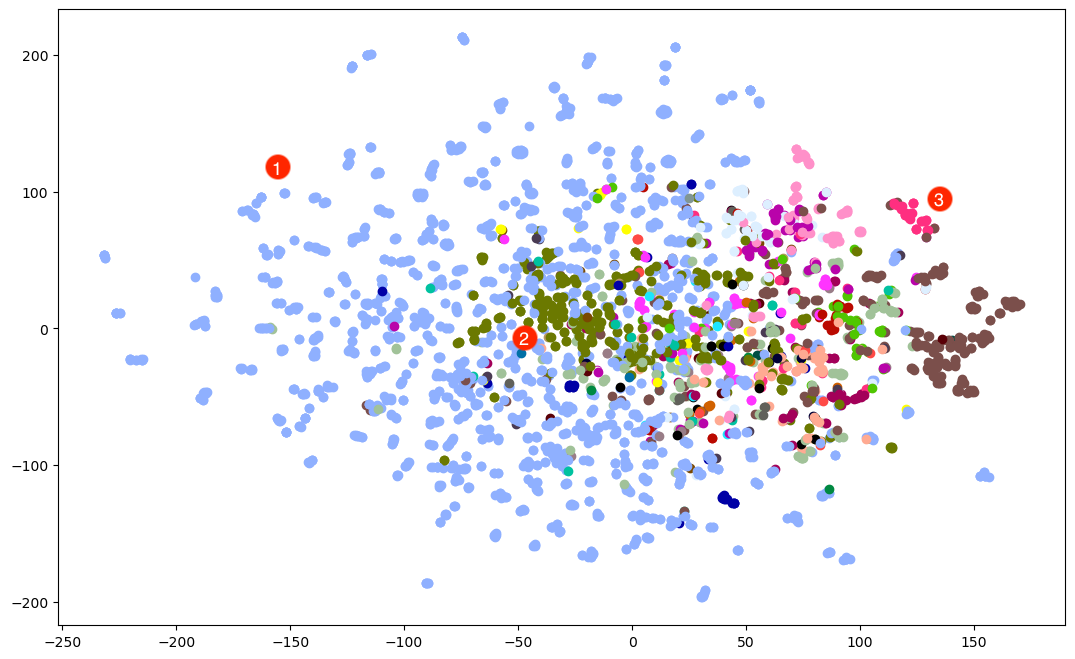
\includegraphics[width=\linewidth]{assets/png/experimentation/categories}}}
    \end{minipage}%
    \begin{minipage}{.4\textwidth}
        \centering
        \subfloat[\centering \texttt{x-apisguru-categories} Word Cloud]{{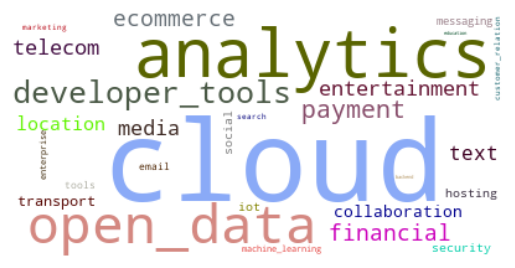
\includegraphics[width=\linewidth]{assets/png/experimentation/cloud}}}
    \end{minipage}

    \caption{Visualization of APIs.guru Dataset by Category and Semantic Relationship}
    \label{fig:documents-plot}
\end{figure}

\section{Approach}\label{sec:approach}
When dealing with OpenAPI Specifications, we are working with JSON or YAML files (which are structured).
Moreover, these files follow the OpenAPI Specifications; thus we know that the documents will contain a very similar structure. \\ \\
Since we are dealing with a very high number of documents, it is paramount to have a fast and reliable index that can be searched through.
For this reason, we decided to use vector embeddings to represent documents in our database.
Embedding models offer a way of transforming documents into vectors of numbers, and -- in our case -- we used Google's Universal Sentence Encoder~\cite{cer_universal_2018} to perform the aforementioned task.
The embedding is done on only a part of the document's content, namely everything that is contained in the~\verb|description|, \verb|name|, \verb|title|, and \verb|summary| tags. \\ \\
We chose to do so because these tags are the only ones that contain natural language descriptions of the API in general or of its endpoints.
After the creation of the embeddings, we saved the vectors -- as well as the name, version, and id -- of the specifications in an Elasticsearch index.
We chose Elasticsearch and the ELK (Elastic-Logstash-Kibana) stack because it is very rapid and scalable.
Moreover, Elasticsearch offers the possibility of searching documents based on the \textit{K}-NN algorithm. \\ \\
This solution seems to be the most promising for the amount of data and hardware availability we have for this project.
We were considering also deep-learning models but discarded them since they are resource intensive and would be overkill for this kind of application.
\section{Ground Truth}\label{sec:ground-truth}
To evaluate the performance of our information retrieval system, we used a ground truth.
Our ground truth consists in a textual file in which we have a query and the expected result.
Some examples are depicted in Figure~\ref{fig:ground-truth}.\\ \\
The file is divided into blocks of two lines.
The first line represents the query that will be vectorized and passed to the $K$-NN query.
On the other hand, the second line represents the title of the document that needs to be found in the top 5 results of the query.
The title of the document on the second line of the block has been chosen manually, this means that we read some of the API specifications and wrote a query that can be connected to that specific document. \\ \\
However, in some cases, there can be multiple documents that satisfy one query; for example, in the case of the query \("\)driving license registration service.\("\)
In the database, there are several different APIs related to the query mentioned: \("\)Transport Department, Tamil Nadu\("\) and \("\)Transport Department, Haryana.\("\)
In such cases, we take the first occurrence that starts with the words \("\)Transport Department.\("\)

\begin{figure}[!h]
    \centering
    \begin{verbatim}
             ...
             aws iot service on secure tunneling
             AWS IoT Secure Tunneling

             driving license registration service
             Transport Department

             sentiment analysis service api
             Text Analytics & Sentiment Analysis API | api.text2data.com

             email mailbox checker
             MailboxValidator Free Email Checker
             ...
    \end{verbatim}
    \caption{Ground Truth}
    \label{fig:ground-truth}
\end{figure}
\section{Evaluation}\label{sec:preliminary-evaluation}

\subsection{Method}\label{subsec:method}
To evaluate the performance of our solution, we used average precision and recall.
In information retrieval systems~\cite{canamares_offline_2020}, precision is defined as the inverse of the position in which the document -- defined in the ground truth -- was found in (Equation~\ref{eq:precision}).
Where $POS$ is the position in which the document was found in ($1$ to $5$ if the document is in the top $5$, $0$ otherwise).
\begin{equation}
    P_i = \frac{1}{POS_i}
    \label{eq:precision}
\end{equation}
The average precision is the average of the precisions among all queries defined in the ground truth (Equation ~\ref{eq:avg-precision}).
Where $N$ is the total number of queries in the ground truth.
\begin{equation}
    \overline{P} = \frac{1}{N} \cdot \sum^N_{i=1}P_i
    \label{eq:avg-precision}
\end{equation}
Finally, the recall is defined as the number of documents found in the top $5$ -- regardless of the position they were found in -- over the total number of queries (Equation~\ref{eq:recall}).
Where $C$ is the number of documents found in the top $5$, and $N$ is the total number of queries in the ground truth.

\begin{equation}
    R = \frac{C}{N}
    \label{eq:recall}
\end{equation}

\subsection{Results}\label{subsec:results}
The results obtained with the embedding + K-NN solution are very promising, as we can see in the t-SNE plot (Figure~\ref{fig:tSNE-plot}, Subsection~\ref{fig:tSNE-plot}). \\ \\
With the \("\)Y\("\) markers representing the queries, and the dots representing the most similar documents found for that query, we can see that the dots and \("\)Y\("\) markers of the same colors are fairly close to each other. \\ \\
Moreover, we performed a validation step with a ground truth.
From the validation step, we concluded that the average precision and recall of the document retrieval are:
\[\overline{P} = 0.6 ~~~~~~ R = 1.0\]
This validation was done on 10 different queries.
The position in which each ground truth appeared in the searches can be found in Figure~\ref{fig:ground-truth-eval}.

\begin{figure}[!h]
    \centering
    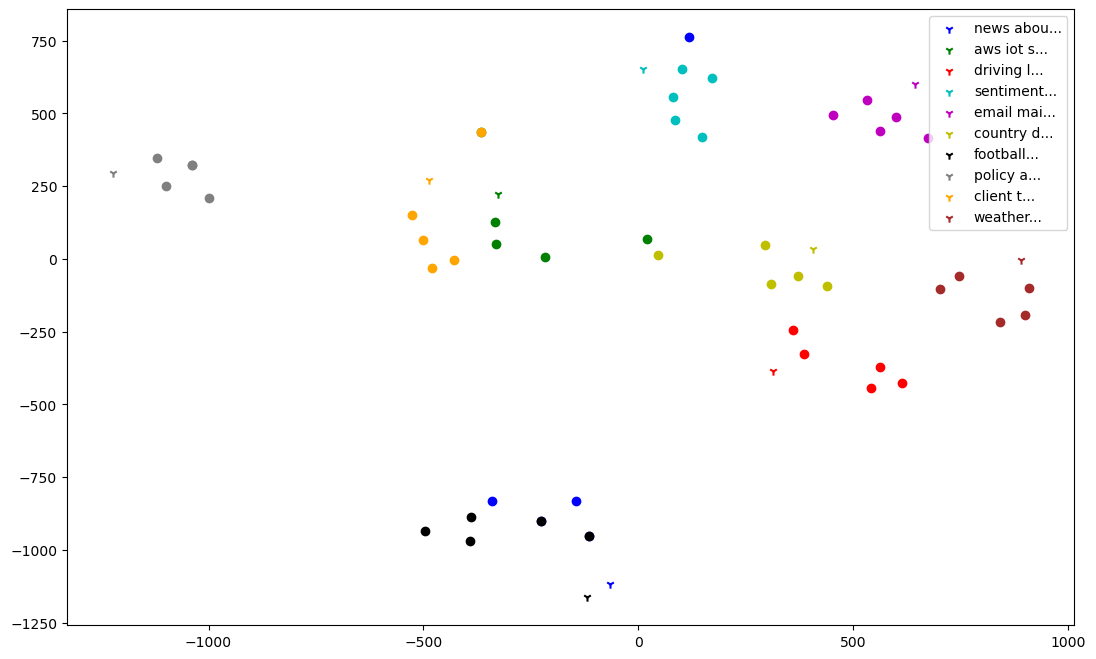
\includegraphics[width=13cm]{assets/png/experimentation/sne}
    \caption{t-SNE Plot}
    \label{fig:tSNE-plot}
\end{figure}

\begin{figure}[!h]
    \begin{verbatim}
  Position in which the ground truth was found:

      "NFL v3 Ply-by-Play" was found at position #1
      "AWS IoT Secure Tunneling" was found at position #4
      "Transport Department" was found at position #4
      "Text Analytics & Sentiment Analysis API | api.text2data.com" was
        found at position #4
      "MailboxValidator Free Email Checker" was found at position #1
      "Interzoid Country Data Standardization API" was found at position #1
      "Soccer v3 Projections" was found at position #1
      "PolicyClient" was found at position #1
      "NetworkManagementClient" was found at position #3
      "Interzoid Get Weather City API" was found at position #2
    \end{verbatim}
    \caption{Ground Truth Evaluation}
    \label{fig:ground-truth-eval}
\end{figure}

\noindent As we can see, all ground truths we found in the top 5 results -- hence $R = 1.0$.
The validation on the ground truth, though, does not paint the full picture of the capabilities this solution offers.
For example, Figure~\ref{fig:query-example} represents the top 5 documents returned by the information retrieval system if we try searching using the query: \("\)american sports news\("\). \\ \\
As we can see in Figure~\ref{fig:query-example}, the engine is able to recognize that both the \textit{NFL} and the \textit{MLB} are professional American sports leagues.
The former being the National Football League, and the latter being the Major League Baseball.
Moreover, it is also able to understand that soccer is a sport and return it. \\ \\
As can be seen both in the average precision ($\overline{P} = 0.6$), and the above example, there are still some noisy results that match part or none of the queries, but this is acceptable.
The reason is that this is not the only means of searching.
To further filter the documents returned by the information retrieval system, we will implement a DSL for the user to specify filters to apply to the output of the natural language query.

\begin{figure}[!h]
    \begin{verbatim}
            These are the top 5 results of the query "american sports news":

                1. NFL v3 Play-by-Play     v.1.0   [67%]
                2. News Plugin             v.1     [66%]
                3. Soccer v3 Projections   v.1.0   [64%]
                4. MLB v3 Projections      v.1.0   [64%]
                5. NFL v3 Scores           v.1.0   [64%]
    \end{verbatim}

    \caption{Example Output of a Query}
    \label{fig:query-example}
\end{figure}
\section{Comparison}\label{sec:comparison}
After validating our system against a tailored ground truth, we compared the results of API Scout with the ones of APIs.guru.
The comparison was performed by taking the queries from the ground truth and searching for them on the APIs.guru website.
The result of this evaluation is depicted in Figure~\ref{fig:apis-guru-eval}.
APIs.guru was not able to yield any document for any of the queries given.
For this reason, APIs.guru's platform has an average precision ($\overline{P}$) of 0 and a recall ($R$) of 0.

\begin{figure}[!h]
    \begin{verbatim}
          Position in which the ground truth was found:

              "NFL v3 Ply-by-Play" was NOT found
              "AWS IoT Secure Tunneling" was NOT found
              "Transport Department" was NOT found
              "Text Analytics & Sentiment Analysis API | api.text2data.com" was
                NOT found
              "MailboxValidator Free Email Checker" was NOT found
              "Interzoid Country Data Standardization API" was NOT found
              "Soccer v3 Projections" was NOT found
              "PolicyClient" was NOT found
              "NetworkManagementClient" was NOT found
              "Interzoid Get Weather City API" was NOT found
    \end{verbatim}
    \caption{APIs.guru Evaluation}
    \label{fig:apis-guru-eval}
\end{figure}

